\ifdefined\included
\else
\setcounter{chapter}{8} %% Numéro du chapitre précédent ;)
\dominitoc
\faketableofcontents
\fi

\chapter{The director task: Assessing cognitive architectures}
\chaptermark{The director task}
\minitoc

The contribution presented in this chapter is excerpted from our work, submitted to the RO-MAN 2021 conference. This contribution closes this thesis and has been achieved in collaboration with other PhD students of the HRI teams. Guilhem Buisan was concerned about the task planning part. Amandine Mayima worked on the supervision component. Kathleen Belhassein has designed the presented task with us giving her psychologist point of view to create a task on which user studies could be performed. The engineer Yannick Riou worked on the motion planning component allowing us to develop a task where the robot acts on its environment. My concern about this task has been the integration of my previous contributions about Ontology and the REG. It has also been the opportunity to create an entire architecture extending the ones presented all along with this thesis and linked with the contributions of the team. Finally, I contribute to the Situation assessment component and on the Language understanding part.

The components related to my teammates will be briefly described to give an overview of the architecture. The newly introduced capabilities on which I work will be more detailed to explain the links I make between all my contributions, centred on the knowledge representation.

\section{Introduction}

Developing robotic architectures adapted to Human-Robot Interaction and thus able to carry out interactions in an acceptable way is still today a real challenge. The complexity comes, among other things, from the number of capabilities which the robot must be endowed with and therefore from the number of software components which must be integrated in a coherent manner. Such architectures should provide the robot with the capability to perceive its environment and its partners, to merge and interpret this perceptual information, to communicate about it, to plan tasks with its partner, to estimate the others' perspective and mental state, etc. Once developed, evaluating these architectures can be difficult because all these components grouped into a single system. The tasks we usually want the robot to handle must highlight a maximum of abilities, while still being simple enough to be reproduced by the community. Moreover, we should be able to conduct user studies with it to validate choices regarding naive users.

Since a long term goal of the robotic field is to see robots evolving in our daily life, many tasks and scenarios have been inspired by everyday activities. Even if these tasks offer a large variety of situation to ba handle since the human partner is not limited in its actions, they have the disadvantage of not highlighting some subtle abilities which are nevertheless necessary for good interaction.
The robot guide task \cite{satake_2015_should} in mall, museum, or airport, requires high communication skills to understand free queries (possibly involving chatting) and respond to them, whether to indicate a direction or to give advice. However, the perception needs can be limited due to the vast environments, as well as the perspective-taking needs due to the same perception of the environment by the robot and the human\footnote{For sure we can find some tricky cases where it could help but they do not reflect common situations.}. Finally, with such a task the human partner is not an actor of the task and just has to listen to the robot once their question is asked. Even if being in more constrained environments, bartender-like tasks~\cite{petrick_2012_social} have the same disadvantages. Indeed, the human is considered as a customer, and as such, the interaction with the robot is limited. The robot will never ask the human to help it for performing a task and their actions do not require coordination either full collaboration.

To involve the human partner in the task and requiring him to act with the robot, assembly-like tasks~\cite{tellex_2014_asking} can be used. Nevertheless, in most cases, the human acts as an assistant rather than as a partner as full collaboration can be challenging to perform. The robot thus elaborates a plan and performs the assemble, then asks for help when detecting errors during the execution (e.g., when it cannot reach some pieces). Here the task leads to unidirectional communication. Moreover, because in such a task both the robot and the human have equivalent knowledge about the environment, it can be hard to design situations where belief divergence appear and thus perspective-taking would be required.

Scaling down an everyday task to transform it into a toy task around a table can deduce the task complexity and allow easy reproducibility. Moreover, it allows making the robot and the human work in the vicinity of each other, with smaller robots for example. With the toy version of the assembly task presented in~\cite{brawer_2018_situated}, the human is more involved in the task. They ask the robot to take pieces and to hold them to help them assemble a chair. Even if the communication is unidirectional, we could imagine inverting the roles to test different abilities. Moreover, communication implies objects referring with the use of various visual features about the entities. Even if both agents have the same knowledge about the environment, the communication is grounded according to the current state of the world. In this task, no decision has to be made by the robot but once again, inverting the roles could open other challenges.

To focus studies around perspective-taking and belief management, the Sally and Anne scenario, coming from a psychology test, has been studied in robotic~\cite{milliez_2014_framework}. In this scenario, the robot is a spectator of a situation where two humans come and go from a room, and move an object from a box to another. Since a human is in the room when the other is acting, a belief divergence appears between the two humans and the robot has to understand it. While the task highlights the belief management, it is first limited regarding the perspective-taking since the human presence or not could be sufficient to estimate the humans beliefs\footnote{When both humans are in the room they have the same perception of the scene but have different beliefs about hidden objects. Perspective-taking would be required if the humans could lean over the boxes to check what is inside.}. Moreover, the humans do not act with the robot since it is just a spectator of the scene. In addition, no goal is formulated and the human neither interacts with one another. Finally, no communication is needed in the task. The scenario is thus focussed on the analyse of a situation.

In this chapter, we first propose a new psychology-inspired task that we think to be challenging for the Human-Robot Interaction community and rich enough to be extended: the Director Task. Inter alia, it requires perspective-taking, planning, knowledge representation with theory of mind, manipulation, communication, and decision-making. Then, we present the robotic cognitive architecture that we develop to perform the task in its nominal cases. Finally, on the basis of the presented task and what has been developed, we present a discussion about the possible future challenges and evaluations for the research community, with possible extensions of the task.

\section[From psychology to Human-Robot Interaction]{The Director Task: From psychology to Human-Robot Interaction}

In this section, we present the origins of the Director Task and the needs it aims to respond to regarding other tasks from the psychology. We then detail the setup we have designed in terms of objects characteristics and organisation in the environment. We end this section with our adaptation and the required abilities we have identified.

\subsection{The original task}

The Director Task has been mainly used in psychology researches as a test of the Theory-of-Mind usage in referential communication. This task originates from a referential communication game from~\cite{krauss_1977_social}. In this game, two participants are one in front of the other with an opaque panel between them. A speaker as to describe odd designs to a listener, either to number them for the adults or create a stack of cubes for the children. To refer to the odd figures, participants have to use images (e.g. "it looks like a plane").

This game was then adapted by Keysar et al.~\cite{keysar_2000_taking} and become the Director Task. It has been used to study the influence of mutual knowledge in language comprehension. In this task, two people are placed one in front of the other but instead of an opaque panel between them, they place a vertical grid composed of different cells and objects in some cells. The \textbf{director}, a participant or in most cases an accomplice, instructs the \textbf{receiver}, a participant, about objects to move in the grid. The receiver thus follows the director's instructions about objects to move. The particularity of the task is that some cells are hidden from the director meaning that the receiver, being on the other side of this grid, does not have the same perspective as the director. He thus knows the content of more cell than the director and consequently sees more objects. When the director instructs the receiver to move an object, for a successful performance, participants must take the perspective of the director to move the right one. Because the configuration evolves all along with the task, he has to update this estimated perspective all along with the interaction.

\begin{figure}[ht!]
\centering
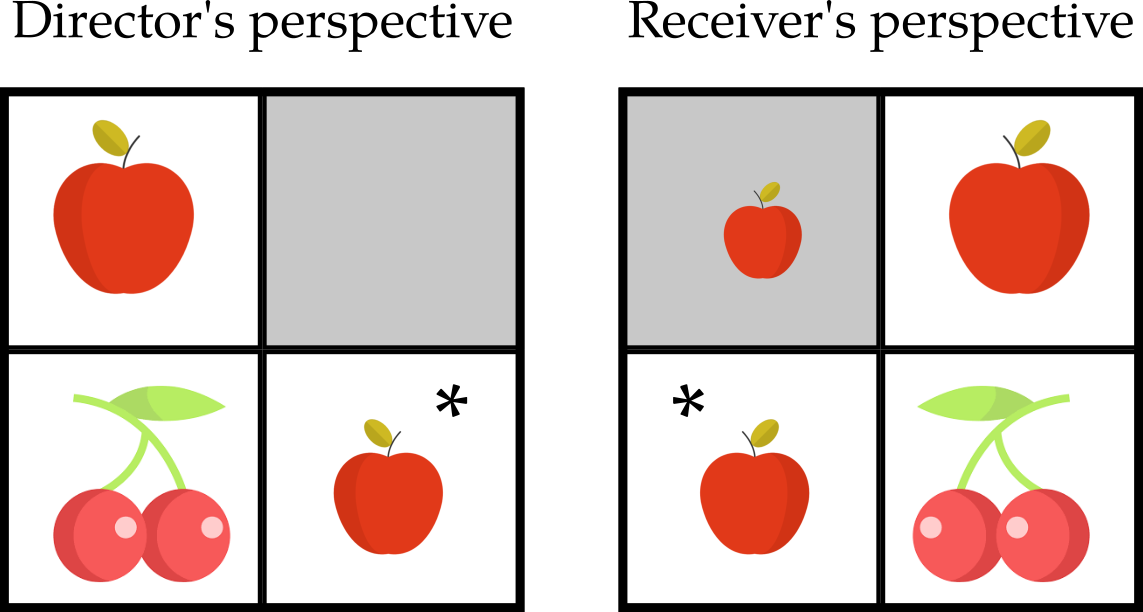
\includegraphics[scale=0.25]{figures/chapter9/dt_apple.png}
\caption{\label{fig:chap9_dt_apple} Sample display from the director's and the receiver's perspectives. The asterisk indicates the target object. Giving the sentence "the smallest apple" the receiver should find the good one even if he can see a smallest one in its perspective. }
\end{figure}

Taking the example of figure~\ref{chap9_dt_apple}, if the director instructs the receiver to take the smallest apple, the target object in its perspective is the one marker with the symbol *. However, for receiver, in its perspective, the target object is not the smallest apple since the smallest one (called distractor) is only visible by the participant and not by the director. The participant then must understand the director's perspective to take the target apple and not the distractor. Some studies showed that for their first attempt, participants took the smallest apple from their own point of view and only after, the target one. These results were interpreted in~\cite{keysar_1994_illusory, keysar_1998_egocentric, keysar_2002_self, keysar_2003_limits} as the participants understanding language in an egocentric way. Some social cognition studies used a computer-version of the Director Task~\cite{dumontheil_2010_online} whose results are consistent with the ones mentioned previously, namely that participants do not use Theory-of-Mind inferences in language interpretation.

Although Theory-of-Mind and perspective-taking both require the attribution of mental states to others, some authors trend at distinguising Theory-of-Mind tasks and perspective-taking tasks as involving distinct although related mechanisms. In~\cite{santiesteban_2012_training}, they considered in their study that perspective-taking abilities were measured by the Director Task whereas Theory-of-Mind usage was investigated through another task called ``strange stories''~\cite{happe_1994_advanced}. This Theory-of-Mind task requires the attribution of mental states to a story protagonist, meaning to maintain an estimation of others' mental states. At the difference, the Director Task requires for adopting the perspective of the director in order to follow their instructions, meaning to use this knowledge in order to execute the task properly. 
In this way, the authors estimated that the Director Task requires a higher degree of self-other distinction by continuously isolating our own perspective from the director one, in order to use them to act. In addition to perspective-taking abilities, the Director Task makes use of executive functions~\cite{rubio_2017_director} (i.e. vary the processing of information according to current goals in an adaptive manner) and attentional resources~\cite{lin_2010_reflexively}.

To summaryse,the Director Task has been used to study referential communication, language comprehension, and perspective-taking abilities. However, to our knowledge, it has never been exploited in the context of a HRI although this task presents interesting challenges for this field. More than technical challenges, it provides a way to investigate the different cognitive and behavioral processes involved in such a cooperative Human-Robot task.

\subsection{The Director Task setup}

The material used in this task has been chosen to be easily acquired and can be hand-built. It is composed of twelve blocks, twelve compartments, and one storage area, each equipped with AR-tags allowing the robot to perceive them without advanced perception algorithms.

%\begin{figure}[b!]
%\centering
%\includegraphics[scale=0.03]{images/material.JPG}
%\caption{\label{fig:material} Part of the material used for the Director Task. Each element is equipped with AR-tags allowing their detection by the robot. Each block has four visual characteristics: a main color, a border color, a geometric figure  and a figure color. }
%\end{figure}

As shown in Fig.~\ref{fig:setup}, the blocks have a primary color covering them all. On two opposite faces, additional visual features are drawn. The top part of these faces is dedicated to the robot's perception with unique AR-tag on each face\footnote{because the tags are different on each side, the director can not refer to them as the receiver does not see the same ones}. The bottom part is the same on both faces and is dedicated to the human perception with a main color, a border, and a geometric figure. Every visual feature (the colors and the forms) has exactly two variants. The colors are either blue or green and the figures are either a triangle or a circle.
The figures and colors have been chosen in such a way to allow the emergence of ``coded words'' between the participant to identify a block. With a bit of imagination, some could refer to the left-most block through the sentence ``the mountain in the sea'' or the second leftmost by ``the puddle''.
The number of features has been chosen to have sixteen block variants from which we remove the four uni-color variants (all the elements having the same color) to avoid too easy description of the kind ``the fully green block''.
Regarding their description complexity, while the main color is directly related to a block, the other colors are respectively related to the border and the figure. This means that for two blocks whose only difference is the color of one of these elements, the said element has to be referred to by its color. A description of a block involving all its features would be ``the [color] block with the [color] border and the [color] [figure]''. Such complete descriptions are hard for the human to process. In this way we expect the participants to minimize the complexity of their communication by referring to the blocks only using the features distinguishing them from other blocks.

Three types of compartment exist. Some are open on two of their opposite sides allowing both the receiver and director to see the content and to manipulate it. Some are open only on one of their sides meaning that only one of the participants can see and take what is inside. The other participant can thus neither know if a block is inside or not. The last compartment type has an open side and the opposite one equipped with a wire mesh. Because of the side with the wire mesh, both participants can see what is inside but only one of them can take it. With these three types, we will be able to test the impact of the awareness of the blocks (e.g., a block is known to be present but not necessarily visible), the visibility of the blocks, and their reachability (e.g., a block can be visible but not reachable).

Finally, one storage area, corresponding to the place where the receiver has to store the blocks, is delimited by a rectangle on a shelf.

\subsection{The adapted task}

\begin{figure}[ht!]
\centering
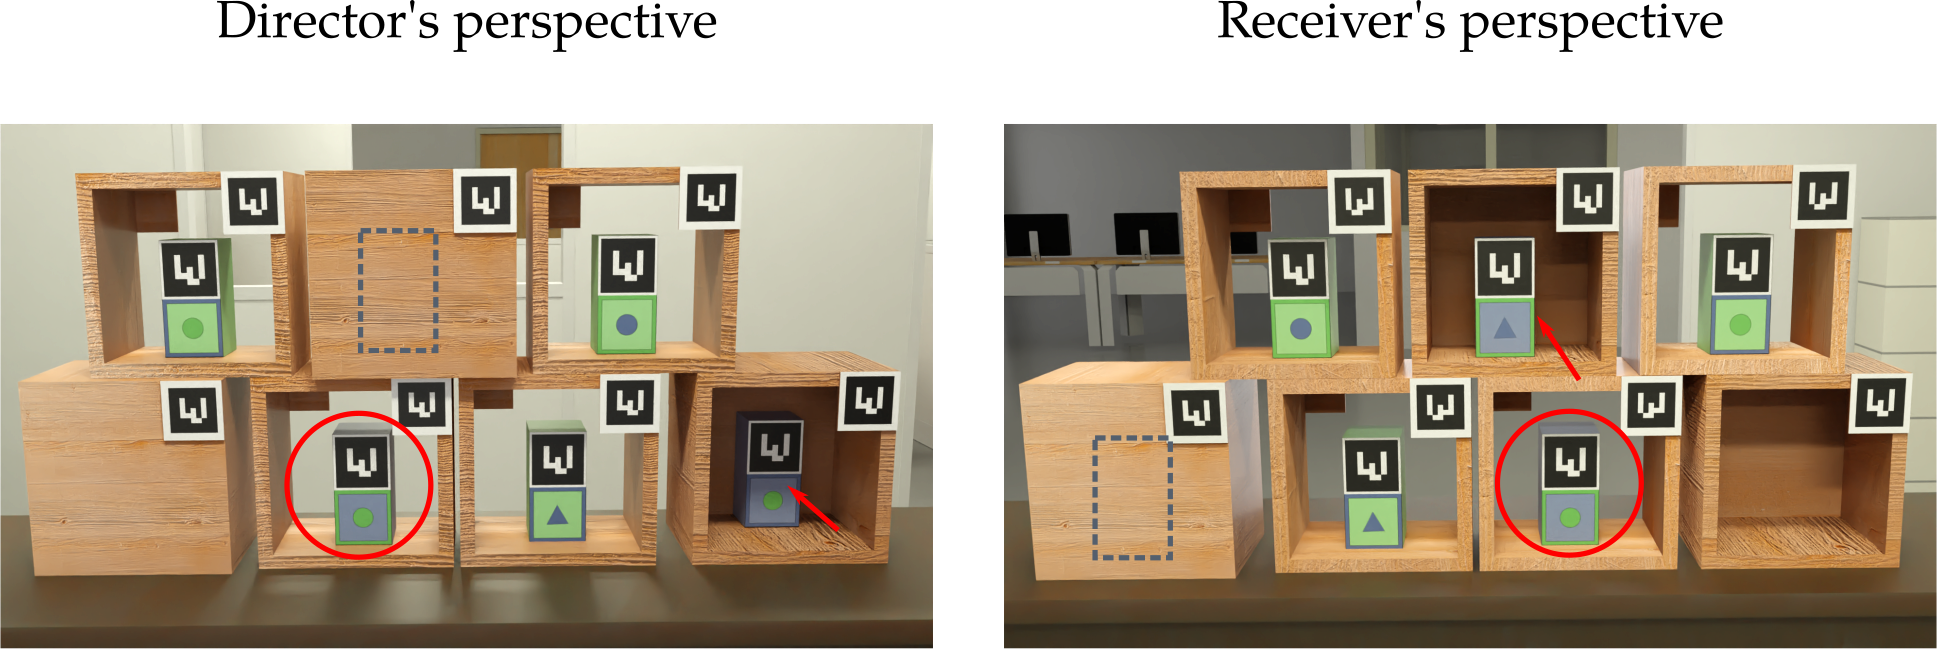
\includegraphics[width=\textwidth]{figures/chapter9/setup.png}
\caption{\label{fig:chap9_setup} A director task setup adapted to the HRI with the director's and receiver's perspectives. For the material, each element (blocks and compartment) is equipped with AR-tags allowing their detection by the robot. Each block has four visual characteristics: a main color, a border color, a geometric figure, and a figure color. Compartments can be hidden for the director or the receiver. For the director to designate the block marked with a red circle, estimating the receiver's perspective, he can refer to it by its main color (blue) because he estimates the other blue block is not visible by the receiver. For the receiver, by taking into account the director's perspective, he can understand the referred block as he estimates the other blue block to not be visible by the director.}
\end{figure}

\section{The cognitive architecture and the knowledge link}

\begin{figure}[ht!]
\centering
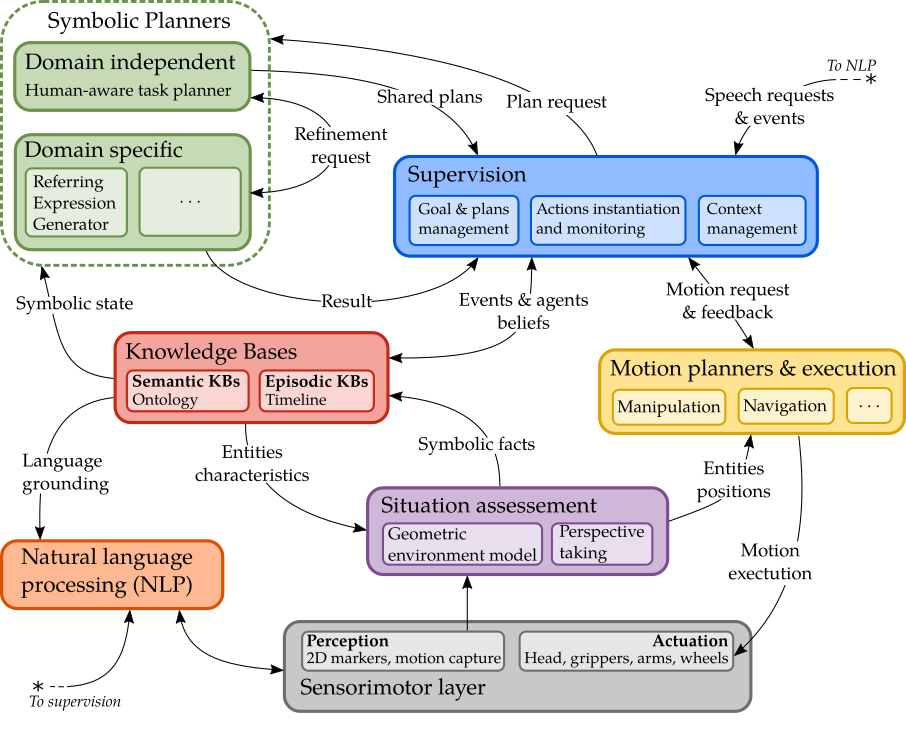
\includegraphics[width=\textwidth]{figures/chapter9/architecture.png}
\caption{\label{fig:chap9_architecture} An overview of the cognitive architecture developed to handle the Director Task. Each block does not necessarily represent one software component but rather an architectural module (in terms of the features it implements). The arrows represent the type of information exchanged between the modules. This architecture extends the ones presented all along with this thesis.}
\end{figure}

\subsection{The declarative memory}

\subsection{The Situation Assessment}

\begin{figure}[ht!]
\centering
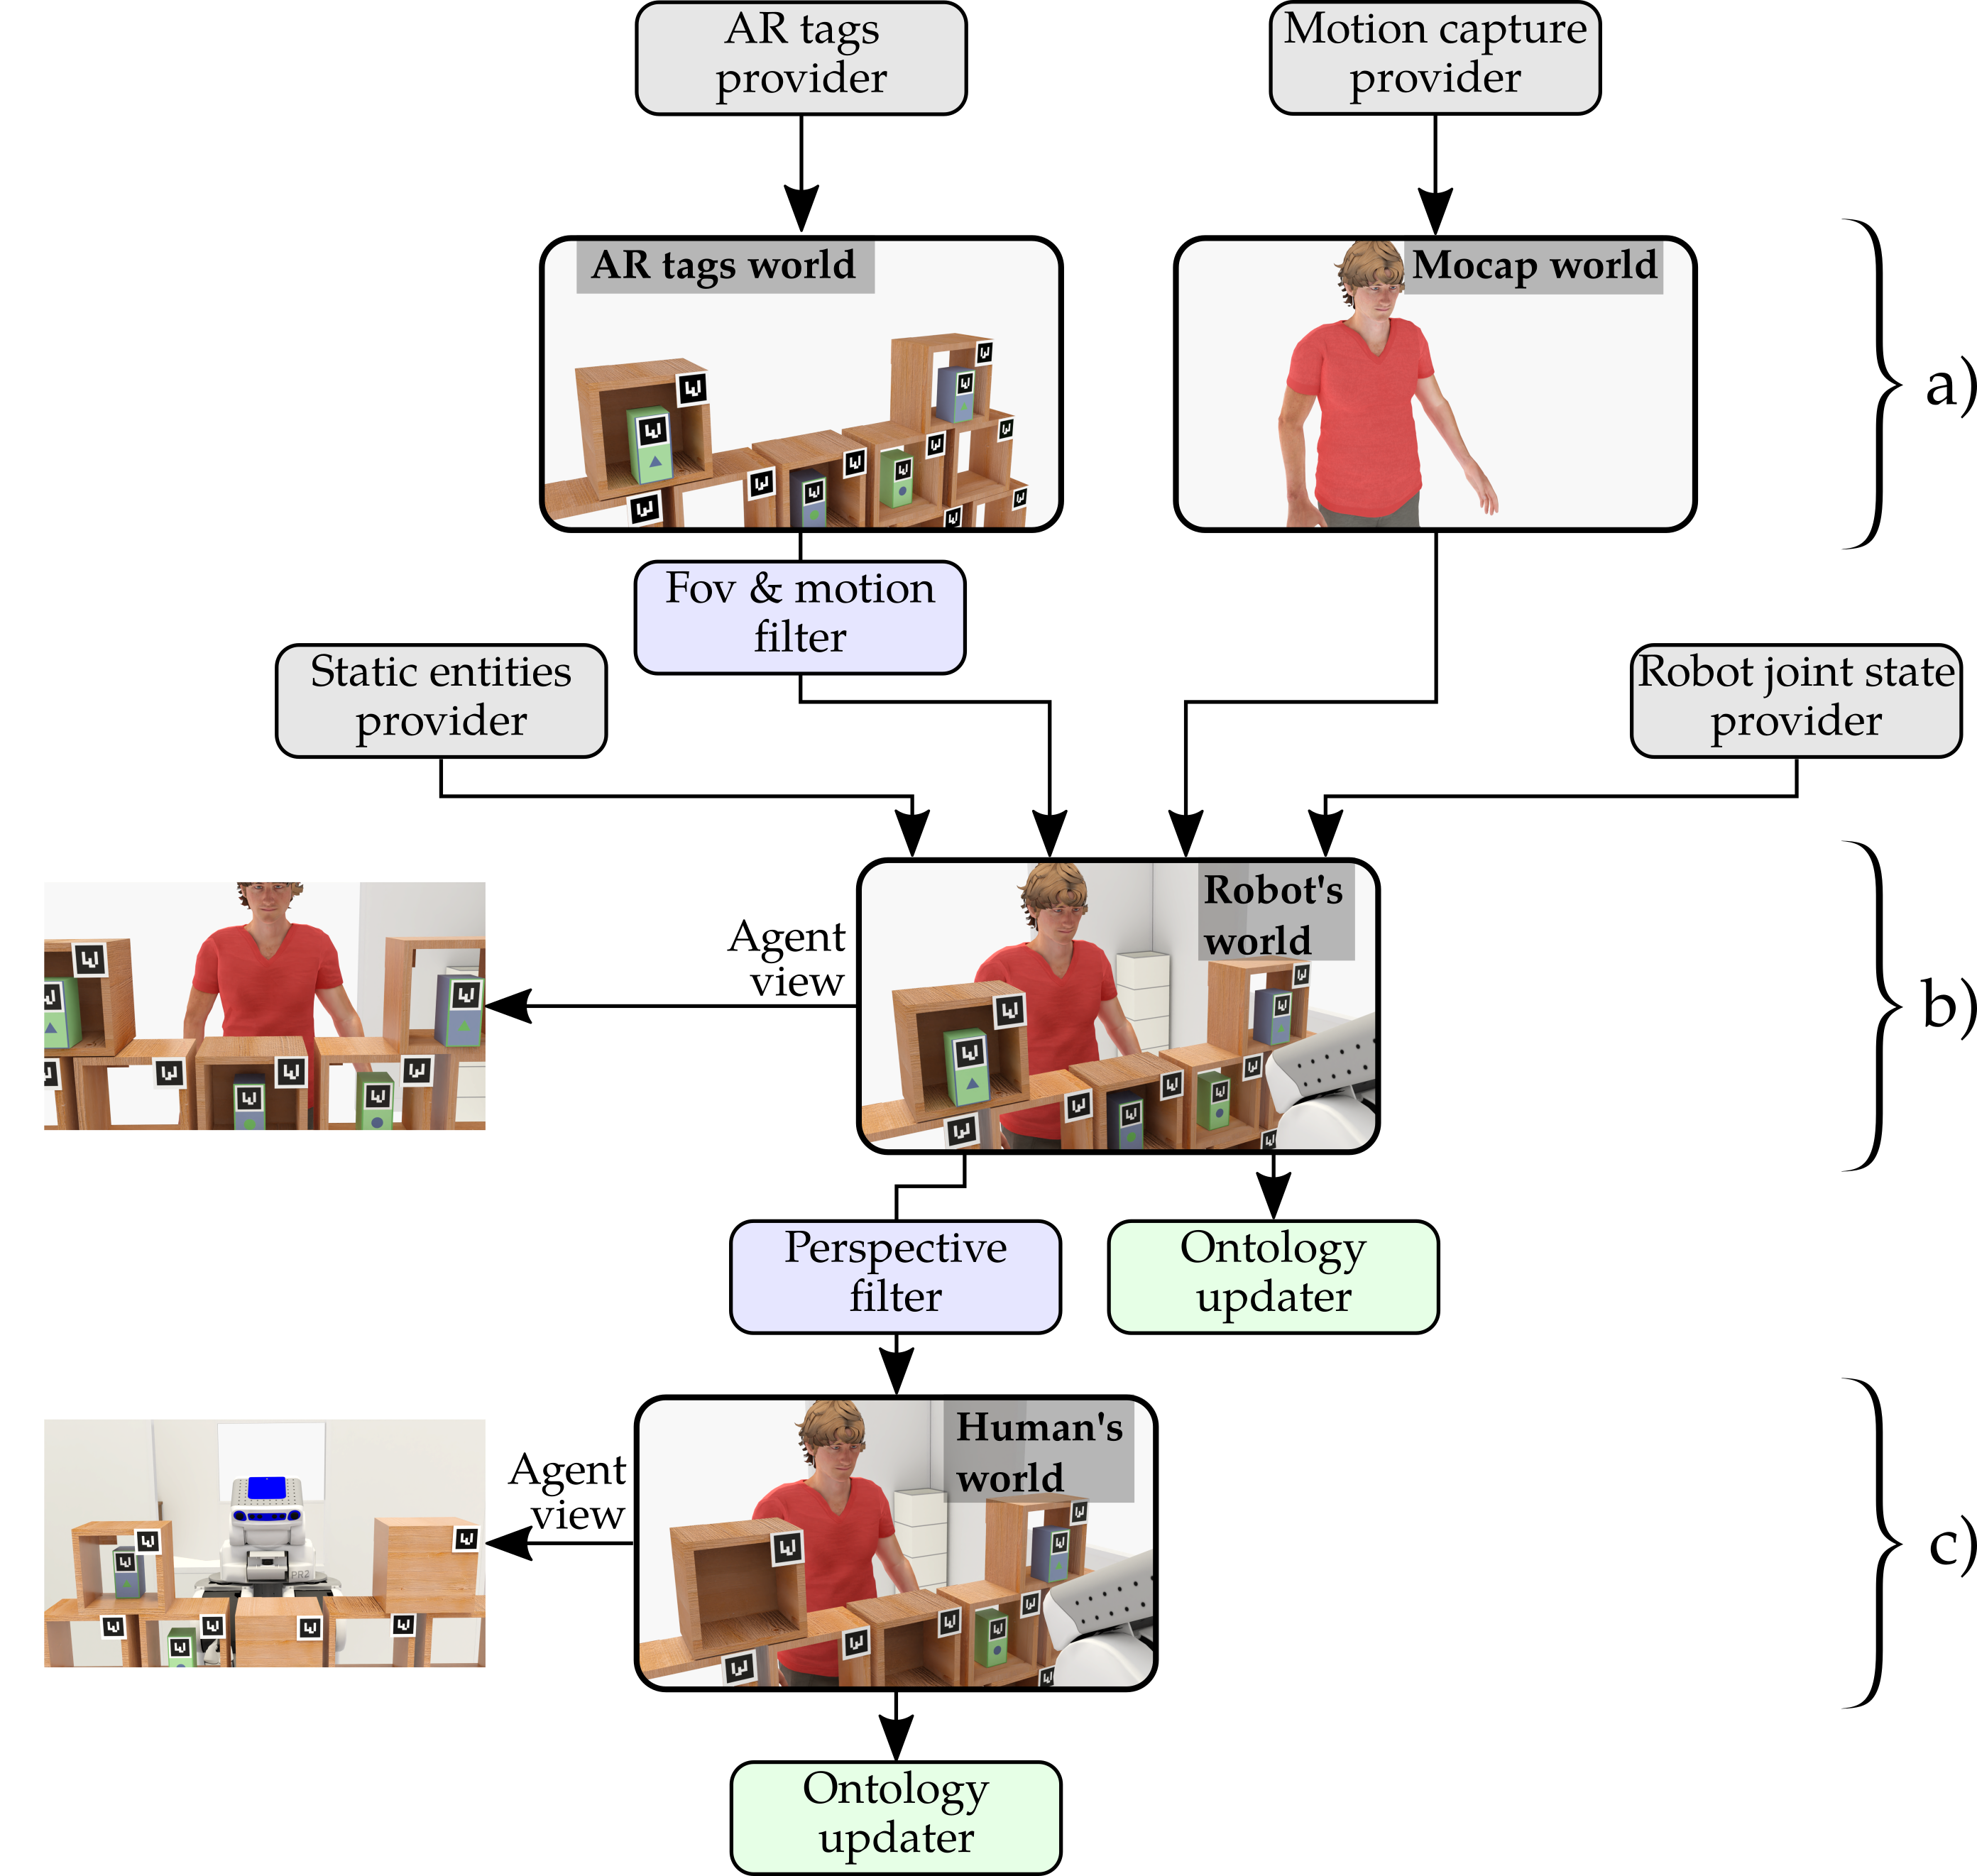
\includegraphics[width=\textwidth]{figures/chapter9/uwds/uwds.png}
\caption{\label{fig:chap9_uwds} The world cascading structure of the geometrical situation assessment system. The two worlds at the top (a) are build from the perception systems and filtered. The world of the middle (b) merges the different perception information and computes symbolic facts on it. The world at the bottom (c) is the estimation of the human world representation and is computed from perspective-taking in the robot's world. Like for the world of the middle, symbolic facts are computed and sent to the semantic knowledge base.}
\end{figure}

\subsection{The supervision}


\section{Integration on a robotic system}

\subsection{The integrated features}

\subsection{Future developments}